\documentclass[letterpaper,10pt,titlepage,journal,compsoc,draftclsnofoot,onecolumn]{IEEEtran}
\linespread{1}
\usepackage{graphicx}                                        
\usepackage{amssymb}                                         
\usepackage{amsmath}                                         
\usepackage{amsthm}                                          

\usepackage{alltt}                                           
\usepackage{float}
\usepackage{color}
\usepackage{url}
\usepackage{listings}

\usepackage{balance}
\usepackage[TABBOTCAP, tight]{subfigure}
\usepackage{enumitem}
\usepackage{pstricks, pst-node}

\usepackage{geometry}
\usepackage{titling}
\geometry{textheight=8.5in, textwidth=6in}


\newcommand{\cred}[1]{{\color{red}#1}}
\newcommand{\cblue}[1]{{\color{blue}#1}}

\usepackage{hyperref}
\usepackage{geometry}

\def\name{Garrett Amidon}


%% The following metadata will show up in the PDF properties
\hypersetup{
  colorlinks = true,
  urlcolor = black,
  pdfauthor = {\name},
  pdfkeywords = {cs461 ''Senior Capstone''},
  pdftitle = {CS 461 Senior Capstone: Problem Statement},
  pdfsubject = {CS461 Senior Capstone},
  pdfpagemode = UseNone
}

\title{Energy Effeciency Center Website \\
	\large Sofware Requirements Specifications}
\author{Garrett Amidon, SR Kanna, James O'Neal}

\begin{document}
\begin{titlingpage}
    \maketitle
	\centering{}
    \begin{abstract}
        
        OSU’s Energy Efficiency Center help manufacturing and industrial companies increase their productivity and reduce their energy footprint by producing reports for energy and productivity recommendations. These reports, projects and funds are maintained in their website. The website has been developed and maintained by several programmers. As a result, the website has become disorganized, difficult to update and use. In order to remedy these issues we will design a secure, user friendly website with good code practices for the Energy Efficiency Center. 	Furthermore, the website is not accessible from mobile devices which decreases productivity while on the job site. With enough time, we would like to create a secure mobile app for the client which they are able to remotely access.
        
    \end{abstract}
\end{titlingpage}

\newpage

\tableofcontents{}

\newpage

\section{Introduction}

\subsection{Purpose}

The purpose of this document is to describe the specific requirements for the Energy Efficiency Center’s (EEC) website. This is the first website release, designed with the intention to provide a secure, user-friendly website with the client requested features. Covered under this document is the project scope, software specifications, user interface, and system features.

\subsection{Product Scope}

EEC helps businesses in the Northwest save money, energy and improve their environmental impact by identifying opportunities to save energy and increase productivity, while reducing cost and waste. The EEC is looking to store and organize the information produced, stored, and tracked through the center’s day to day activity. In order to be most useful to the center, the website needs to be secure and efficiently organized with specific features to manage employees, projects, and clients.\par
The primary features the client is looking to implement can be subdivided into keeping track of projects and employees. Specifically, all active employees should be listed and have account specific details such as such as email, contact, weekly hours, major, the date the started at the center. Furthermore, the website should keep record the number of hours an employee has worked on a task, specifically to keep track of task progress and to prevent employees from exceeding the maximum number of hours. Projects should be monitored from the creation to the completion of the project. Each project should be able to add tasks. There should also be an efficient implementation for tasks not associated with a specific project, which are specific to an employee. Stretch goals such as mobile web application or additional features will be added and evaluated based on the development process. 

\subsection{Definitions}

\begin{tabular}{ | l | l | }
\hline
	EECS & Energy Efficiency Center \\ \hline
	Implementation Call & Calling the client a year after sending the proposal \\ \hline
	Project & Created each time we perform an assessment on a company \\ \hline
	Task & each project has tasks that need to be done along the project \\ \hline
	Management Team & The group, including the stakeholder, who manages other employees \\ \hline
	Exceeds flag & a notification when an employee has exceeded the time allotted for a task \\ \hline
	Assessment & an evaluation of a company looking to reduce its energy output and increase its efficiency \\ \hline
\end{tabular}

\subsection{References}

IEEE 830-1998

\subsection{Overview}

The remainder of the document will go in depth about the following items:
\begin{itemize}
\item Features the website must do
\item Non-functional requirements
\item Design restraints on the website
\end{itemize}

\section{Overall Description}

\subsection{Product Perspective}

The EEC website is intended to be a secure, efficiently organized website to help store and organize the information at the center, specifically with features to manage projects and employees. It is intended to be a self-contained environment with access to wifi which only requires a desktop/laptop with a web-browser, without any external hardware dependencies. There is an existing website in place, but it does not meet the client’s security or usability satisfaction.

\subsubsection{System Interfaces}

The website is mostly a self-contained and does not rely on external hardware. Since the system is web-enabled, the interfaces will be installed through the hardware. The website will be expected on run on the client’s browser of choice. As this is purely as web-based application and not mobile, it will only be available through laptops. The two interfaces required on the system-server is network interface to a network with internet connection and a database connection to the mySQL database containing user and schedule data. As a stretch goal, we will create a web-based mobile application. 

\subsubsection{User Interfaces}

All user interfaces are through the web page.

\subsubsection{Hardware Interfaces}

There are no hardware interfaces

\subsubsection{Software Interfaces}

There are no software interfaces

\subsubsection{Communication Interfaces}

Not currently applicable. 

\subsubsection{Memory Constraints}

Since it is not hardware dependent, there are no hardware memory constraints. There should be enough memory in the laptop/desktop to run our application, but this is a minimal constraint.

\subsection{Design Constraints}

Not currently applicable.

\subsubsection{Operation}

Not currently applicable.

\subsubsection{Site Adaptions and Dependencies}

Not currently applicable.

\subsection{Product Functions}

Specifically, all active employees should be listed and have account specific details such as such as email, contact, weekly hours, major, the date the started at the center. Furthermore, the website should keep record the number of hours an employee has worked on a task, specifically to keep track of task progress and to prevent employees from exceeding the maximum number of hours. Projects should be monitored from the creation to the completion of the project. Each project should be able to add tasks. There should also be an efficient implementation for tasks not associated with a specific project, which are specific to an employee. Stretch goals such as mobile web application or additional features will be added and evaluated based on the development process. 

\subsection{User Characteristics}

The only users who have access to the website are authorized users, or employees. They will have access through a portal through Oregon State, through which they enter their credentials. Specific employees will have more authority than others which are associated with their credentials. This authority allows them to create projects, tasks, add additional hours etc.

\subsection{Design and Implementation Constraints}

There are a few constraints to consider during development: passwords must be sent and stored in encrypted form and data must be stored in a relational database for quick queries. Furthermore, we are limited to free, open-source technology. The website will be maintained by the customer’s organization, so all code and software should be easy to use and maintainable to them. We have agreed to use primarily use Bootstrap, HTML, CSS, Javascript, PHP and SQL.

\subsection{Apportioning Requirements}

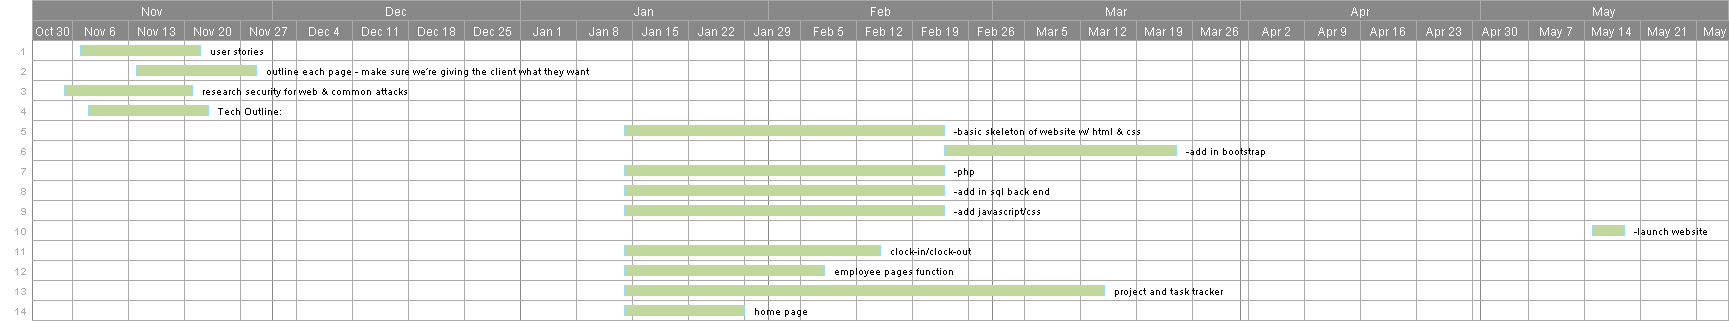
\includegraphics[scale=0.25]{RequirementsDocument}

\subsection{Assumptions and Dependencies}

We assume that the operating system and browser running the website is up to date and can handle new CSS, Javascript plugins etc. We also assume there is stable, secure internet connection available.

\section{Specific Requirements}

\subsection{Log Hours}

\subsubsection{Description and Priority}

Logging hours is how employees report what they have spent time on. This is self reported. It allows them to record how much time they have worked and bill hours to specific tasks. The management team will use this system to understand which employees need help completing a task. Additionally, this time tracker ensures no employee exceeds a set amount of hours on any given task. The priority of this system is high as it is necessary to accomplish work on a daily basis.

\subsubsection{Action and Result}

This amount will be assigned to one or more tasks resulting in a total hour count the employee has spent on each task. If assigning hours to a task results in an employee exceeding their allotted time for that task, the employee will be notified.

\subsubsection{Functional Requirements}

The functional requirements for this system are as follows:
\begin{itemize}
\item Allow user to assign hours to a single task
\item Allow user to split hours between multiple tasks
\item Detect if employee has exceeded hour limit on a given task
\item Include the date and a description
\end{itemize}

\subsection{Employee Information}

\subsubsection{Description and Priority}

All information about employees must be made available. Each employee has a name, major, start date, and contact information. These items should be displayed on their employee page. The priority of this system is medium as it will not make the site unusable if it does not exist.


\subsubsection{Action and Result}

The action of a user selecting an employee will result in the display of all relevant information. The action of an employee selecting themselves will result in the display of their information and an option to edit this information. 

\subsubsection{Functional Requirements}

The functional requirements of this system are as follows:
\begin{itemize}
\item Allow user to select an employee
\item Allow user to edit their information
\item Allow user to view information about employee
\end{itemize}

\subsection{Projects and Tasks}

\subsubsection{Description and Priority}

A project begins when the assessment of another company begins. A project ends once an implementation call has been placed. A task is an item that needs to be completed. A task can be connected to a project or exist by itself. Both projects and tasks have start and end dates which can be manipulated. This system is a method for viewing, tracking, and manipulating past, present, and future projects and tasks. Each task has information about that task associated with it which can be viewed and edited. The priority of this system is high due to its necessity for organization within the EEC.

\subsubsection{Action and Result}

The action of creating a project will result in a new viewable project with a start and end date. The action of editing the project will result in the extension or reduction of the project deadline. The action of creating a task will result in a new viewable task. The action of assigning a task to a project will result in that task being connected to the project. The action of selecting a task will allow information about that task to be viewed and updated. The action of editing the task will allow end date, allotted hours, and projects it is connected to to be changed.

\subsubsection{Functional Requirements}

The functional requirements for this system are as follows:
\begin{itemize}
\item Allow all tasks to be viewed and edited
\item Allow all projects to be viewed and edited
\item View all tasks connected to a project
\item Create a project or task
\item Connect a task to a project
\item Disconnect a task from a project
\item View information related to a task	
\end{itemize}

\subsection{Home Page}

\subsubsection{Description and Priority}

The home page or profile page for a given user will be a central place to access the most important aspects of the website. Things included here will be links to all other pages. The home page will only be accessible by those who have logged in with a valid user-name and password. The home page is an area where important data will be readily available. The priority of this system is high because without it users will be lost.

\subsubsection{Action and Result}

The action of logging in successfully will result in the user viewing their profile page. The action of selecting a link on the homepage will result in the user being taken to the connected page. The action of selecting home will take the user back to the homepage. 

\subsubsection{Functional Requirements}

The functional requirements for this system are as follows:
\begin{itemize}
\item A central hub where all pages are accessible
\item An always available button that brings the user back to the homepage
\item A method for logging out
\end{itemize}

\section{Nonfunctional Requirements}

\subsection{Performance Requirements}

The EEC website must function consistently and quickly. The site cannot crash or become unusable. This is important to the site because employees will depend on it in order to complete their daily job. In order to test that these requirements are met we will complete performance tests after the site is complete. We will also beta test the website with the EEC to make sure it can handle daily use.\par
In addition, the website needs to be easily usable. This includes navigation and time to learn. In order to gauge these factors we will use a heuristic evaluation. We will be evaluating the site on user control and freedom, consistency and standards, and recognition rather than recall. Control and freedom is dependant upon user’s ability to control what page they are on and move about the site freely without going through unnecessary pages. Consistency and standards is dependant upon words and actions meaning the same thing on all pages. Recognition rather than recall is dependant upon the user’s ability to intuitively navigate without having to learn and remember.

\subsection{Software Quality}

The software quality of the website must allow for future additions and modifications to the website. These future changes will be made by employees who did not design the original site. For this reason code must be clear and stick closely to one format. Comments will be used heavily in order to increase code readability. The current employees who works on modifying the database and website will verify that the code is understandable once the site is created.

\section{Signatures\newline\newline\newline}

\noindent\begin{tabular}{ll}\newline
\makebox[2.5in]{\hrulefill} & \makebox[2.5in]{\hrulefill}\\
Anya Lehman & Date\\[8ex]% adds space between the two sets of signatures
\makebox[2.5in]{\hrulefill} & \makebox[2.5in]{\hrulefill}\\
Sr Kanna & Date\\[8ex]
\makebox[2.5in]{\hrulefill} & \makebox[2.5in]{\hrulefill}\\
Garrett Amidon & Date\\[8ex]
\makebox[2.5in]{\hrulefill} & \makebox[2.5in]{\hrulefill}\\
James O'Neal & Date\\
\end{tabular}

\end{document}
